\chapter{Extraction de caractéristiques}
\section{Courbure}

Dans ce premier exercice, nous devons implémenter la fonction \texttt{curvature\_hist()} qui prend en paramètre une image et qui retourne un tableau d'histogramme des courbures de l'image. Ces valeurs sont normalisées et sont donc dans l'intervalle [0;1]. Le paramètre \texttt{plot} permet de produire ou non un histogramme.

Voici donc le code de cette fonction :

\lstinputlisting{code/curvature_hist.py}

A la ligne 4, nous appelons la fonction \texttt{curvature()} qui est définie précédemment et qui va calculer le contour et la courbure de l'image (et afficher les images si le paramètre \texttt{plot} est à \texttt{True}.


Si nous appelons donc notre fonction \texttt{curvature\_hist()} avec deux images différentes (ici l'image 1 et 13) et en affichant les histogrammes, nous obtenons les histogrammes de la figure \ref{curvaturehist} ainsi que les deux tableaux de valeurs suivantes :

\vspace{0.6cm}
\small\texttt{[ 0.8175   0.04097  0.01117  0.02235  0.0298   0.03352  0.02142  0.00931  0.00466  0.00186]}

\small\texttt{[ 0.68003  0.11886  0.04461  0.03834  0.11049  0.00662  0.00105  0.       0.       0.     ]}
\vspace{0.6cm}

\begin{figure}[h]
  \centering
    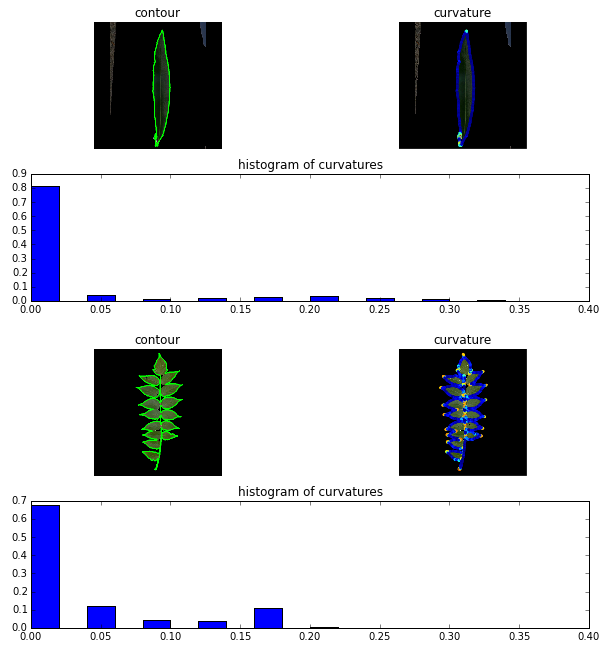
\includegraphics[width=0.6\linewidth]{img/curvatureHist.png}
  \caption{Histogrammes des courbures des images des feuilles 1 et 13}
  \label{curvaturehist}
\end{figure}


\section{Nouvelle caractéristique}

Dans l'exercice suivant, il est question d'extraire une nouvelle caractéristique pour l'ajouter au tableau de l'histogramme créé précédemment. Pour cela nous avons choisi d'extraire l'enveloppe convexe de la feuille et de la comparer avec le contour. La caractéristique est le coutour divisé par l'enveloppe convexe. Cette caractéristique est intéressante car plus la feuille est lisse et convexe, plus la caractéristique sera proche de 1 et plus il y a de renflements, plus la valeur va diminuer. Voici le code de la fonction qui va extraire cette caractéristique : 

\lstinputlisting{code/hull_ratio.py}


\section{KNN}

Il faut à présent utiliser les caractéristiques pour entraîner et évaluer un classifieur KNN. Pour ce faire, nous devons d'abord charger toutes les images et leur extraire les caractéristiques qu'on met dans un tableau. Il faut également créer un vecteur qui contient les classes de chaque image pour pouvoir entraîner notre classifieur. Ensuite nous séparons nos données en données d'entraînement et de test. A la fin, nous entraînons le classifieur. Voici le code qui permet toutes ces étapes : 

\lstinputlisting{code/knn.py}



Dans ce code, nous avons défini que 40\% des données allaient servir de données de test. Et nous avons instancié le classifieur KNN à K = 3. Nous pouvons changer la valeur de K pour voir si nous obtenons de meilleurs résultats.


% Code integration example
%\begin{lstlisting}[language=bash]
%  sudo apt-get update
%  sudo apt-get install drupal7
%\end{lstlisting}

% Image integration example
%\begin{figure}[h]
%  \centering
%    \includegraphics[width=1\linewidth]{img/drupalFirstPage.png}
%  \caption{Page d'accueil du site créé avec Drupal sur une instance EC2}
%  \label{drupalfirstpage}
%\end{figure}
